\documentclass[a4paper, 12pt]{article}
\usepackage[utf8]{inputenc}
\usepackage[russian]{babel}
\usepackage{amsmath}
\usepackage{graphicx}
\usepackage{hyperref}

\title{TEncDM: Понимание свойств диффузионной модели в пространстве кодировок языковых моделей}
\author{}
\date{}

\begin{document}

\maketitle

\begin{abstract}
Представленная работа описывает Text Encoding Diffusion Model (TEncDM) — новаторский подход к моделированию текста с помощью диффузионной модели, работающей в пространстве кодировок языковой модели. В отличие от традиционных методов, основанных на эмбеддингах, TEncDM использует кодировки, которые содержат больше контекстной информации и улучшают качество предсказаний модели. Кроме того, в модели используется трансформерный декодер, специально разработанный для учета контекста при предсказании токенов, а также самоконтроль, что повышает точность генерации текста. Экспериментальные результаты на задачах перефразирования, суммаризации и упрощения текста подтверждают превосходство TEncDM над традиционными неавторегрессивными диффузионными моделями.
\end{abstract}

\section{Введение}
Авторегрессивные модели, такие как GPT-4 \cite{gpt4} и Llama 3 \cite{llama3}, демонстрируют высокое качество в задаче генерации текста. Они создают текст, проходя последовательно по каждому токену, что делает их подход надежным и естественным для создания длинных связных текстов. Однако эти модели имеют два значительных недостатка. Во-первых, они не могут корректировать ошибки, допущенные на ранних этапах генерации. Поскольку авторегрессивные модели генерируют текст слева направо, любая ошибка, допущенная на начальных шагах, будет "разрастаться", искажая весь последующий текст. Во-вторых, авторегрессивный подход требует обработки каждого токена по отдельности, что замедляет процесс генерации, особенно на длинных последовательностях.

Диффузионные модели, активно развивающиеся в таких областях, как генерация изображений, аудио и видео, предлагают альтернативный метод. В диффузионных моделях процесс генерации происходит параллельно, что позволяет генерировать всю последовательность токенов одновременно. Это делает модель более гибкой и позволяет обрабатывать и корректировать любые части текста в процессе генерации, что ускоряет работу. Кроме того, диффузионные модели позволяют сократить количество необходимых вычислительных операций путем дистилляции, что также сокращает время генерации текста.

Существует множество подходов к адаптации диффузионных моделей для текстовой генерации, от замены гауссовского шума на категориальный до обучения на небольших латентных представлениях текста. Однако еще не найден оптимальный подход, который позволил бы эффективно моделировать текст с учетом особенностей его структуры и содержания. В данной работе исследуется возможность обучения диффузионной модели в латентном пространстве контекстуальных кодировок, предоставляемых языковыми моделями. Мы выделили и проанализировали влияние декодера, шумового расписания и метода самоконтроля на качество генерации текста, что позволило сформулировать основные рекомендации по разработке диффузионных моделей для текстовой генерации.

\section{Постановка задачи и принципы диффузионного моделирования}
Задача генерации текста заключается в построении текста, который удовлетворяет заданному условию, например, теме или стилю. Диффузионное моделирование предполагает преобразование случайного шума в структурированный текст. Для обучения модели требуется "прямой процесс диффузии", в котором шум постепенно добавляется к латентному представлению текста, и "обратный процесс", в ходе которого модель обучается восстанавливать исходный текст на основе зашумленного представления. При этом диффузионная модель должна учитывать контекст и структуру текста на всех этапах денойзинга, чтобы восстановить полноценную текстовую последовательность.

\section{Методология}
Методология TEncDM включает несколько ключевых компонентов, которые позволяют повысить качество генерации текста за счет учета контекста и контроля шума на каждом этапе денойзинга.

\begin{figure}[t]
\begin{center}
\centerline{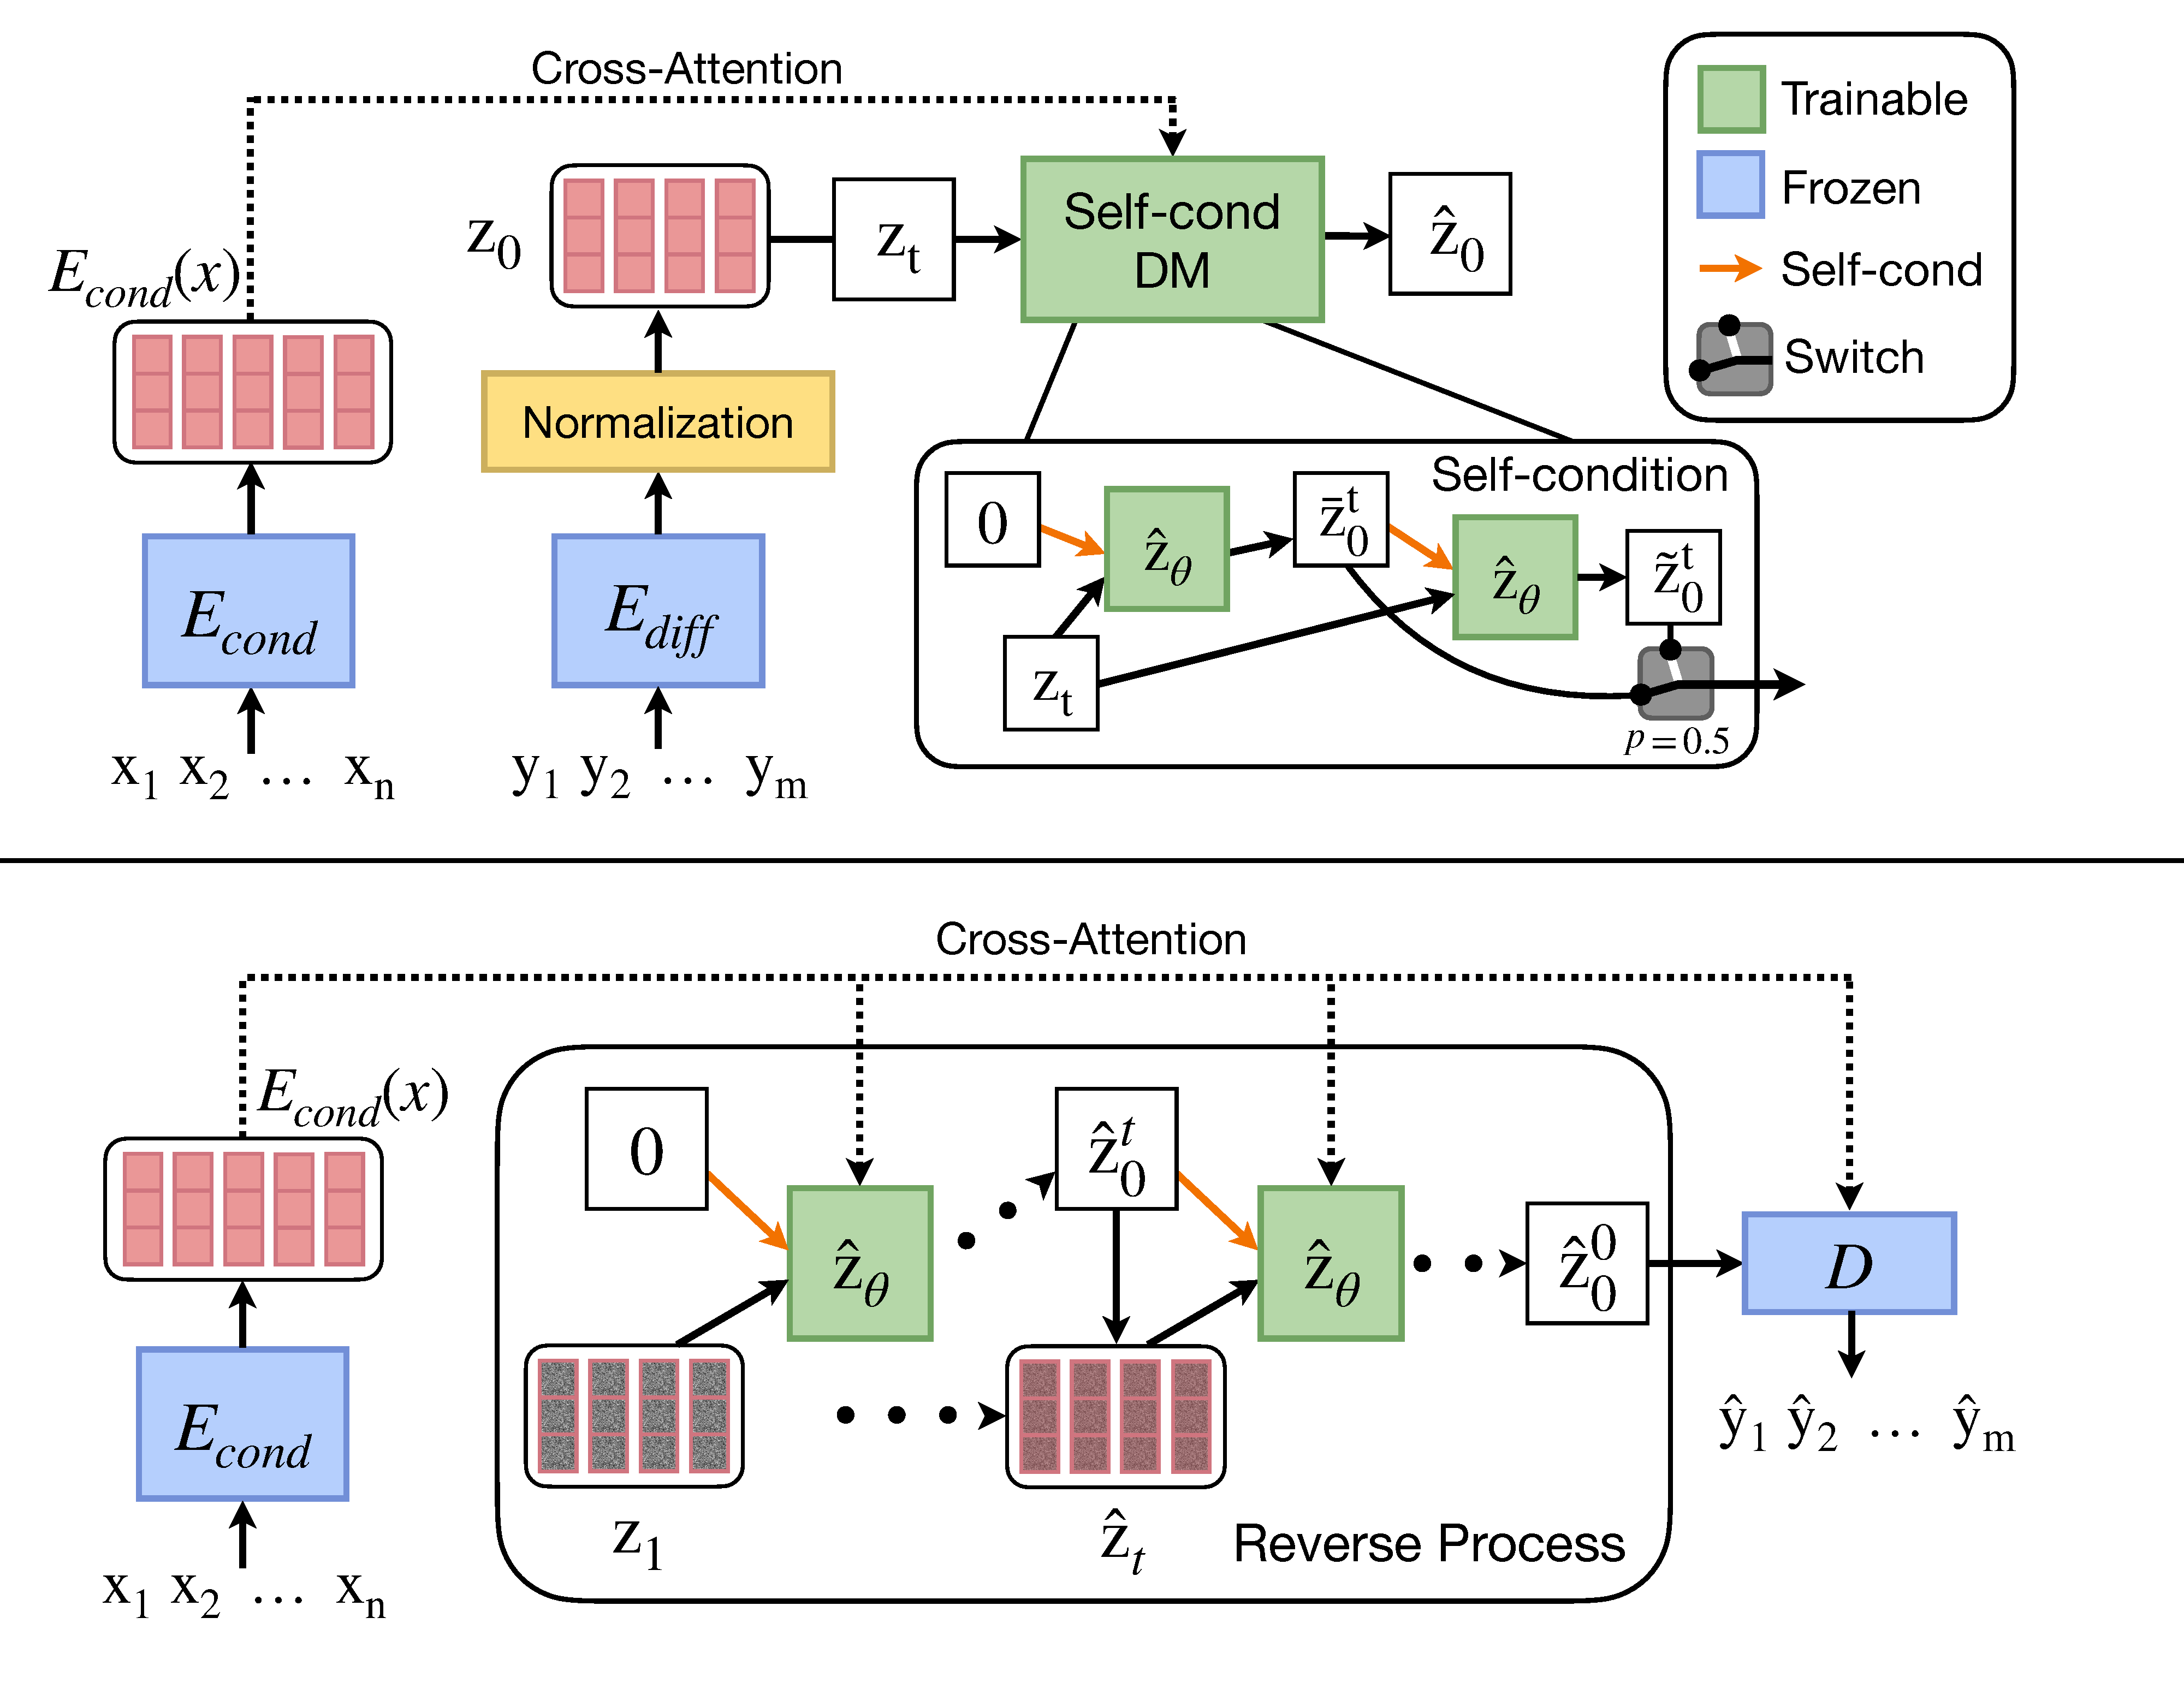
\includegraphics[width=\columnwidth]{images/framework.pdf}}
\caption{Обзор нашего фреймворка для условной генерации. Вверху - процесс обучения, внизу - процесс генерации.}
\label{fig::model_pipeline}
\end{center}
\end{figure}

\subsection{Кодировщик}
TEncDM использует предварительно обученную трансформерную модель для преобразования текста в латентное пространство кодировок, которое содержит контекстную информацию. В отличие от эмбеддингов, которые представляют токены фиксированными значениями, кодировки адаптируются к контексту, в котором находятся, что позволяет модели лучше понимать смысл текста. Кодировщик обрабатывает каждое предложение, преобразуя его в последовательность латентных переменных, выровненных по длине для корректной обработки в модели.

\subsection{Диффузионная модель}
Диффузионная модель TEncDM построена на базе трансформера с 12 слоями и обучается восстанавливать исходные латенты из зашумленных версий. Для этого используется шумовое расписание, в котором интенсивность шума контролируется параметром, что позволяет задать сложность восстановления на каждом шаге. Чем выше шум, тем сложнее диффузионной модели восстановить исходный текст, но это способствует более устойчивому обучению модели. Таким образом, контролируемое добавление шума помогает улучшить точность генерации текста.

\subsection{Декодер}
После этапа денойзинга декодер преобразует восстановленные латенты в текст. В TEncDM применяется трансформерный декодер, который учитывает контекст для каждого токена, что улучшает качество предсказаний. Декодер обучается независимо от диффузионной модели, чтобы его работа не зависела от ошибок, допущенных на предыдущих шагах. Таким образом, даже если диффузионная модель допускает неточность при восстановлении латентов, декодер способен скорректировать результат, улучшив итоговое качество текста.

\subsection{Самоконтроль}
Введение самоконтроля позволяет диффузионной модели повышать точность предсказаний на каждом шаге, ориентируясь на собственные предыдущие предсказания. В модели реализовано два сценария самоконтроля: с нулевым значением (для случаев, когда предыдущая информация отсутствует) и с учетом данных из предыдущего шага. Эксперимент показал, что самоконтроль позволяет модели сократить количество шагов денойзинга, что ускоряет процесс генерации.

\section{Экспериментальный анализ}
Для проверки эффективности TEncDM были проведены эксперименты на задачах условной генерации текста, включая перефразирование, суммаризацию и упрощение текста. Были использованы датасеты QQP \cite{qqp} (вопросы-перефразирования), XSum \cite{xsum} (экстремальная суммаризация) и Wiki-Auto \cite{wiki_auto} (упрощение текста). Модель TEncDM оценивалась на основе следующих метрик:

\begin{itemize}
    \item \textbf{Perplexity} — показатель, который измеряет логарифмическое среднее расстояние между вероятностью предсказания модели и реальными данными. Низкий уровень Perplexity указывает на высокую точность генерации.
    \item \textbf{MAUVE} — метрика, оценивающая близость распределений сгенерированного и референтного текста. MAUVE измеряет, насколько тексты, сгенерированные моделью, похожи на реальные тексты, что позволяет оценить реалистичность и связность.
    \item \textbf{Дивергенция} — метрика, которая измеряет разнообразие текстов, предотвращая дублирование и стандартизацию.
    \item \textbf{Меморизация} — метрика, которая измеряет, насколько модель запоминает данные из обучающего набора, что позволяет предотвратить чрезмерное повторение.
\end{itemize}

\subsection{Результаты экспериментов}

\begin{table}
% \setlength{\tabcolsep}{3pt}
\centering
\begin{tabular}{l|llll}
\hline
\multicolumn{1}{l|}{\textbf{Encoder}}
    & \multicolumn{1}{c}{\textbf{ppl} $\downarrow$} 
    & \multicolumn{1}{c}{\textbf{mem} $\downarrow$}
    & \multicolumn{1}{c}{\textbf{div} $\uparrow$}
    & \multicolumn{1}{c}{\textbf{mauve} $\uparrow$}\\
\hline
\multicolumn{5}{c}{\textbf{ROCStories}} \\
\hline
BERT emb & $48.9_{.36}$ & $.371_{.003}$ & $.324_{.002}$ & $.600_{.016}$ \\
BERT & $29.1_{.89}$ & ${.453}_{.003}$ & ${.295}_{.002}$ & $\textbf{.762}_{.043}$ \\
RoBERTa & $\textbf{28.3}_{.33}$ & ${.443}_{.003}$ & ${.302}_{.002}$ & ${.647}_{.019}$\\
T5 & ${31.3}_{.54}$ & $.427_{.003}$ & $.312_{.004}$ & $.706_{.024}$ \\
BART & $34.1_{.52}$ & $.441_{.006}$ & $.299_{.005}$ & $.705_{.030}$\\
\hline
Source text & $21.7$ & $.365$ & $.403$ & $.876$ \\
\hline
\multicolumn{5}{c}{\textbf{Wikipedia}} \\
\hline
BERT emb & $156.1_{1.8}$ & $.263_{.004}$ & $.517_{.002}$ & $.378_{.055}$ \\
BERT & $\textbf{104.4}_{2.1}$ & $.286_{.002}$ & $.504_{.003}$ & $\textbf{.874}_{.011}$ \\
\hline
Source text & $37.3$ & $.122$ & $.615$ & $.957$ \\
\hline
\end{tabular}
\caption{Сравнение энкодеров}
\label{tab::encoders}
\end{table}

\begin{table}
% \setlength{\tabcolsep}{3pt}
\centering
% \resizebox{0.49\textwidth}{!}{
\begin{tabular}{l|cccc}
\hline
\textbf{Decoder} & \textbf{ppl} $\downarrow$ & \textbf{mem} $\downarrow$ & \textbf{div} $\uparrow$ & \textbf{mauve} $\uparrow$ \\
\hline
\multicolumn{5}{c}{\textbf{ROCStories}} \\
\hline
MLP & $39.7_{3.38}$ & $.444_{.002}$ & $.297_{.004}$ & $.716_{.074}$ \\
\; + $Cor(z_0)$ & $31.2_{.33}$ & $.448_{.002}$ & $.293_{.003}$ & $.739_{.051}$ \\
Transformer & $34.2_{.29}$ & $.445_{.001}$ & $.295_{.003}$ & $.714_{.037}$ \\
\; + $Cor(z_0)$ & $\textbf{29.1}_{.89}$ & ${.453}_{.003}$ & ${.295}_{.002}$ & $\textbf{.762}_{.043}$ \\
\hline
\multicolumn{5}{c}{\textbf{Wikipedia}} \\
\hline
Transformer & $180.6_{3.2}$ & $.261_{.001}$ & $.511_{.001}$ & $.526_{.025}$ \\
\; + $Cor(z_0)$ & $\textbf{104.4}_{2.1}$ & $.286_{.002}$ & $.504_{.003}$ & $\textbf{.874}_{.011}$ \\
\hline
\end{tabular}
% }
\caption{Сравнение декодеров}
\label{tab::decoders}
\end{table}

Результаты экспериментов показали, что модель TEncDM превосходит другие существующие подходы в генерации текста по всем основным метрикам. Например, на задаче перефразирования модель показала значительное преимущество перед конкурентами, демонстрируя более точные перефразы при сохранении смысла. На задаче суммаризации модель смогла достичь высоких результатов, генерируя лаконичные и точные резюме. В задаче упрощения текста TEncDM также показала себя лучше других методов, успешно передавая основные мысли сложных текстов в простой форме.

Влияние отдельных компонентов на качество генерации

\textbf{Кодировщик и декодер}. Исследования показали, что использование кодировок вместо эмбеддингов позволяет модели учитывать больше контекста, а продвинутый декодер способен значительно улучшить качество текстов за счет адаптации к особенностям латентного пространства.

\textbf{Самоконтроль}. Анализ показал, что метод самоконтроля увеличивает точность предсказаний модели, особенно при генерации длинных текстов, когда важно учесть каждый шаг для сохранения связности.

\textbf{Шумовое расписание}. Контроль интенсивности шума на каждом этапе улучшил процесс обучения модели и позволил улучшить качество предсказаний, что особенно важно для обработки текстов с неоднородной структурой.

\subsection{Перспективы и ограничения}
Несмотря на высокие результаты, TEncDM имеет ряд ограничений. В частности, процесс генерации замедляется для длинных текстов, так как размерность латентного пространства возрастает. В будущем возможно создание автоэнкодера, который позволит сжимать латенты, улучшая производительность модели. Кроме того, разные задачи требуют настройки параметров модели, что предполагает необходимость в проведении дополнительных исследований для нахождения оптимальных значений для каждого типа задач.

\section{Заключение}
TEncDM демонстрирует высокие результаты в задачах генерации текста, превосходя классические диффузионные и авторегрессивные модели. Работа показала, что переход от эмбеддингов к контекстуальным кодировкам улучшает качество предсказаний и способствует созданию более натуральных текстов. Предложенная модель успешно справляется с различными задачами на реальных данных, показывая универсальность и точность. В дальнейшем планируется улучшить производительность модели за счет уменьшения латентного пространства и оптимизации параметров для различных задач.

\bibliographystyle{plain}
\bibliography{references}

\end{document}
